\documentclass[9pt,mathserif]{beamer}

%% \usepackage{pgfpages}    %%% Notes
%% \setbeameroption{show notes on second screen} %%%%Notes

\usepackage[spanish, es-noshorthands]{babel} 
\usepackage[utf8]{inputenc}

\usepackage{textpos} %textblock
%% \usepackage{tikz,pgfplots}
%% %\setbeamertemplate{navigation symbols}{}

%% %%%%\usecolortheme{rose}
%% %\usecolortheme{seahorse}
%% %\usetheme{Copenhagen}
%% %\usetheme{Warsaw}
\usetheme[width=3\baselineskip]{Berkeley}
\usecolortheme{spruce}   % color verde lindo
\definecolor{forestgreen}{rgb}{0.0, 0.27, 0.13}
\setbeamercolor{itemize item}{fg=forestgreen}
\setbeamercolor{itemize subitem}{fg=forestgreen}
\setbeamercolor{block title}{bg=forestgreen!12,fg=forestgreen}
\setbeamercolor{caption name}{fg=forestgreen}
%% \usecolortheme{beaver}



\usepackage{subfig}
\usepackage{tikz}
\setbeamertemplate{caption}{\raggedright\insertcaption\par}
\setbeamerfont{caption}{size=\scriptsize}
\setlength{\abovecaptionskip}{5pt plus 3pt minus 2pt}
\captionsetup[subfloat]{captionskip=-10pt}

% TITLE PAGE ----------------------------------------------------------------------------------
%\logo{
\includegraphics[width=0.75cm,height=0.75cm]{figuras/ib.png}}

\title[]{MODELADO COMPUTACIONAL DEL COMPORTAMIENTO HIDRODINÁMICO DE ELEMENTOS COMBUSTIBLES NUCLEARES}
\author[]{\large{Julia Martorana, Ezequiel Fogliatto, Federico Teruel, Enzo Dari y Mariano Cantero}}
\institute{\normalsize{Departamento de Mecánica Computacional \\ Centro Atómico Bariloche \\  Comisión Nacional de Energía Atómica \\  Instituto Balseiro - Universidad Nacional de Cuyo}}
\date{}
% -----------------------------------------------------------------------------------------------

\begin{document}
\renewcommand{\tablename}{}                         % Reemplaza la palabra Cuadros, por 'nada' 
\renewcommand{\figurename}{}                        % Reemplaza la palabra Cuadros, por 'nada'

\begingroup
\makeatletter
\setlength{\hoffset}{-.5\beamer@sidebarwidth}
\makeatother
\begin{frame}[plain]
  \titlepage
  \begin{textblock}{5}(-0.5,-0.25)
    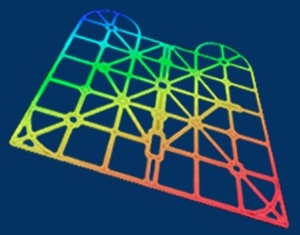
\includegraphics[width=1.15cm]{figuras/ENIEF2017.png}
  \end{textblock}
  \begin{textblock}{5}(12.25,-0.5)
    
\includegraphics[width=1.15cm]{figuras/CNEA.jpg}
  \end{textblock}
  \centering
  \normalsize{XXIII Congreso sobre Métodos Numéricos y sus Aplicaciones} \\
\end{frame}
\endgroup

% -----------------------------------------------------------------------------------------------
% INDICE 
%% \frame[plain]{
%%   \frametitle{Contenidos}
%%   %	\begin{minipage}{\textwidth}
%%    \tableofcontents 
%%   %\end{minipage}
%% }

%% % -----------------------------------------------------------------------------------------------
 \section{Introducción}

\frame{
  \frametitle{Introducción}
  \framesubtitle{Elementos combustibles}

   \begin{minipage}{0.6\textwidth}
    \begin{figure}[!htb]
      \center
      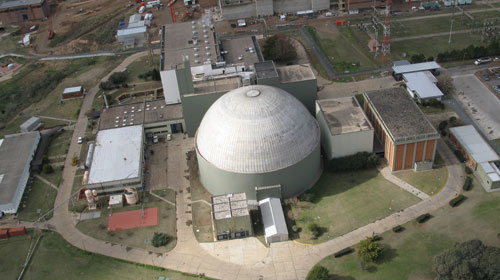
\includegraphics[width=5.25cm]{figsINTRO/atucha2.jpg} \vspace{-2mm}
      \caption{Vista aérea de la Central Nuclear Atucha II.}
    \end{figure}
  \end{minipage}
   \begin{minipage}{0.35\textwidth}
     \vspace{-0.5cm}
    \begin{figure}[!htb]
      \center
      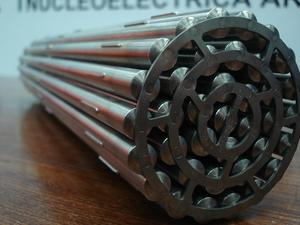
\includegraphics[width=3cm]{figsINTRO/EECC_atuchaI.jpg} \vspace{-2mm}
      \caption{EECC de la CN Atucha I.}
    \end{figure}
  \end{minipage}

  \vspace{-0.5cm}
   \begin{minipage}{0.6\textwidth}
    \begin{figure}[!htb]
    \center
    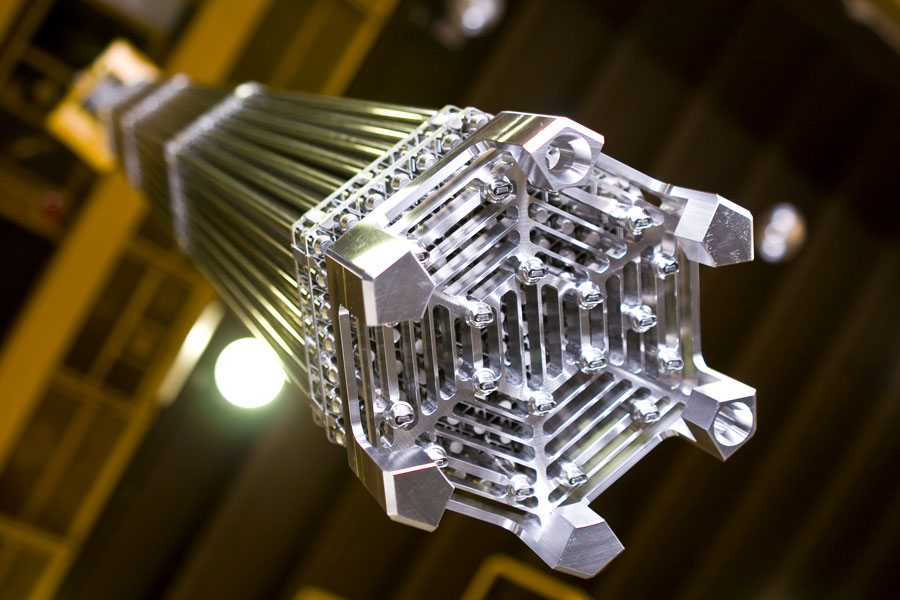
\includegraphics[width=4.75cm]{figsINTRO/CAREMfromCNEAfuelelement.jpg} \vspace{-2mm}
    \caption{Elemento combustible CAREM 25.} 
    \end{figure}
  \end{minipage}
  \begin{minipage}{0.35\textwidth}
    \begin{figure}[!htb]
      \center
      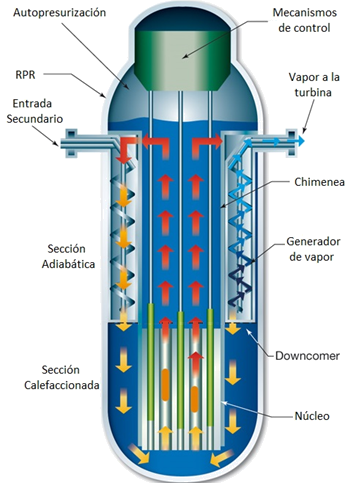
\includegraphics[width=3cm]{figsINTRO/carem.png} \vspace{-2mm}
      \caption{Esquema de funcionamiento del reactor CAREM.[1]}
    \end{figure}
  \end{minipage}
    \footnotetext[1]{\tiny{Laboratorio THI, CAB, CNEA}}
    
  
    \note{

      \begin{itemize}
      \item Una central nucleoeléctrica es básicamente un reactor nuclear que se utiliza para generar energía eléctrica. Las mismas producen vapor que posteriormente mueve una turbina acoplada a un generador eléctrico.
      \item El aumento de la produccion de energia que genera una central nuclear esta asociado con la capacidad de refrigeración de los componentes que conforman el núcle del reactor, en particular de los EECC
       \item Lo que limita la refrigeración de los EECC es el fenómeno conocido como Flujo critico de calor (CHF) que está relacionado con la generación y dinámica del vapor.
        
 
        \end{itemize}

    }
  
    %% \begin{itemize}
    %%   \item Se llevan a cabo cálculos numéricos como complemento de estudios de CNAII en un loop de freón.
    %%   \item Se desea evaluar el desempeño termohidráulico de separadores de CAREM.
    %%   \item El flujo es turbulento, se producen vórtices y se requiere la identificación de puntos calientes.
    %%   \item Fenómeno de flujo crítico de calor, optimización del quemado de EC.
    %% \end{itemize}

  

}

% =====================================================================================================
\frame{
  \frametitle{Introducción}
  \framesubtitle{Loop de Freón - Laboratorio de Termohidráulica - CAB - CNEA}

  \begin{minipage}{0.6\textwidth}
    \begin{figure}[!htb]
      \center
      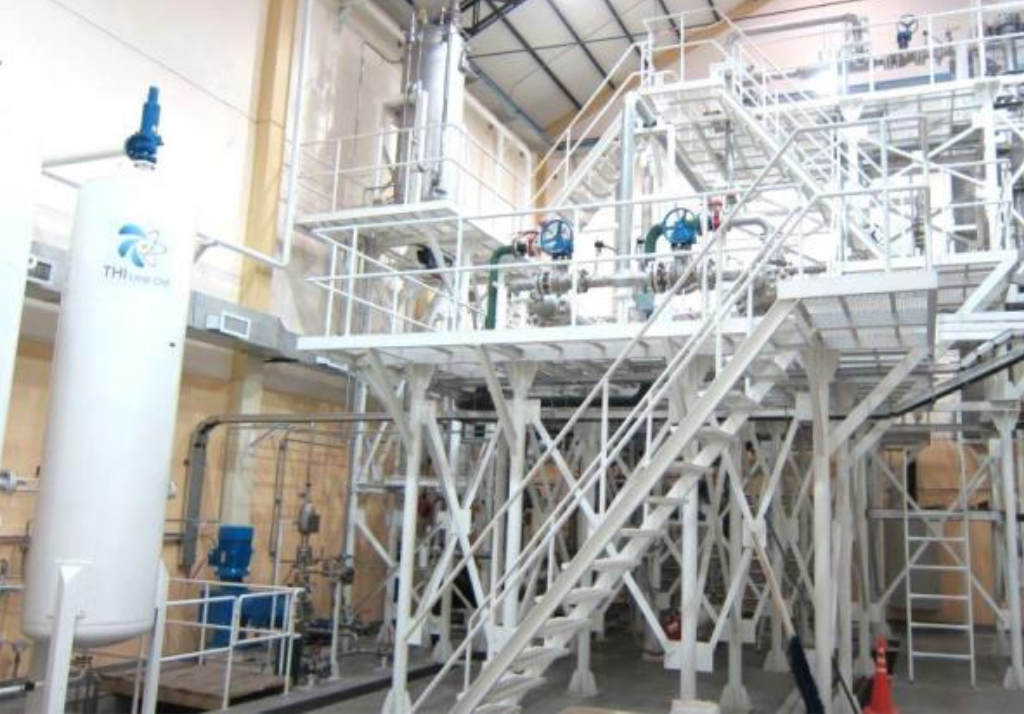
\includegraphics[width=5.5cm]{figsINTRO/freon2b.png}
      \caption{Circuito de ensayos de CHF, Laboratorio THI, CAB.[1]}
    \end{figure}
  \end{minipage}
  \begin{minipage}{0.35\textwidth}
    \begin{figure}[!htb]
      \center
      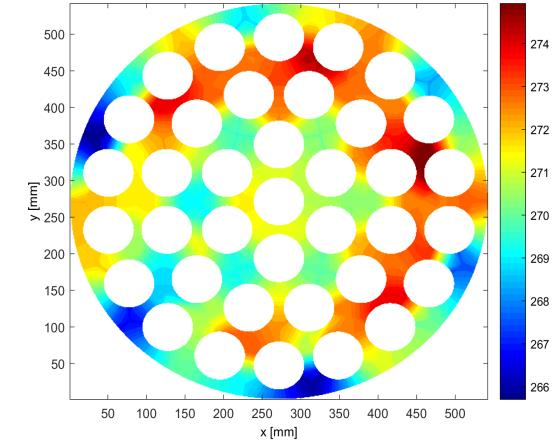
\includegraphics[width=4cm]{figsINTRO/freon4.png}
      \caption{Reconstrucción del perfil térmico en un EC.[1]}
    \end{figure}
  \end{minipage}
  
  \begin{itemize}
  \item Circuito de ensayos para determinar el CHF en EECC.
  \item Posibilidad de ensayar los diferentes diseños de EECC de las centrales nucleares argentinas
  \item Permite llevar a cabo procesos de optimización: incorporar cambios geométricos para mejorar la transferencia térmica.
  \end{itemize}

  \footnotetext[1]{\tiny{Laboratorio THI, CAB, CNEA}}
  
  \note{\begin{itemize}
    \item El circuito de ensayo de CHF...
    \item En la figura se muestra...
      \end{itemize}
  }
  
}

% =====================================================================================================
\section{Objetivos}
\frame{
  \frametitle{Objetivos}

   \begin{block}{Objetivo general}
    Contribuir al desarrollo de la ingeniería y optimización del diseño de elementos combustibles nucleares.
  \end{block}
  %\end{minipage}
  \vspace{1cm}
  
  %\begin{minipage}{0.75\textwidth}
  \begin{block}{Objetivos particulares}
  \begin{itemize}
    \item Realizar cálculos numéricos como complemento de estudios de CNAII en un loop de freón.
    \item Realizar cálculos numéricos para evaluar el desempeño termohidráulico de separadores de CAREM.
  \end{itemize}
  \end{block}
  %\end{minipage}

}

% =====================================================================================================
\section{Herramientas}
\frame{
  \frametitle{Herramientas}
  
  \begin{minipage}{0.5\textwidth}
  \begin{block}{SALOME}
    Programa libre que incorpora módulos para generación de modelos CAD y motores de mallado en 3 dimensiones.
    \begin{itemize}
    \item Representación geométrica detallada de los EC.
    \end{itemize}
  \end{block}
  \end{minipage}
  \begin{minipage}{0.45\textwidth}
     \begin{figure}
     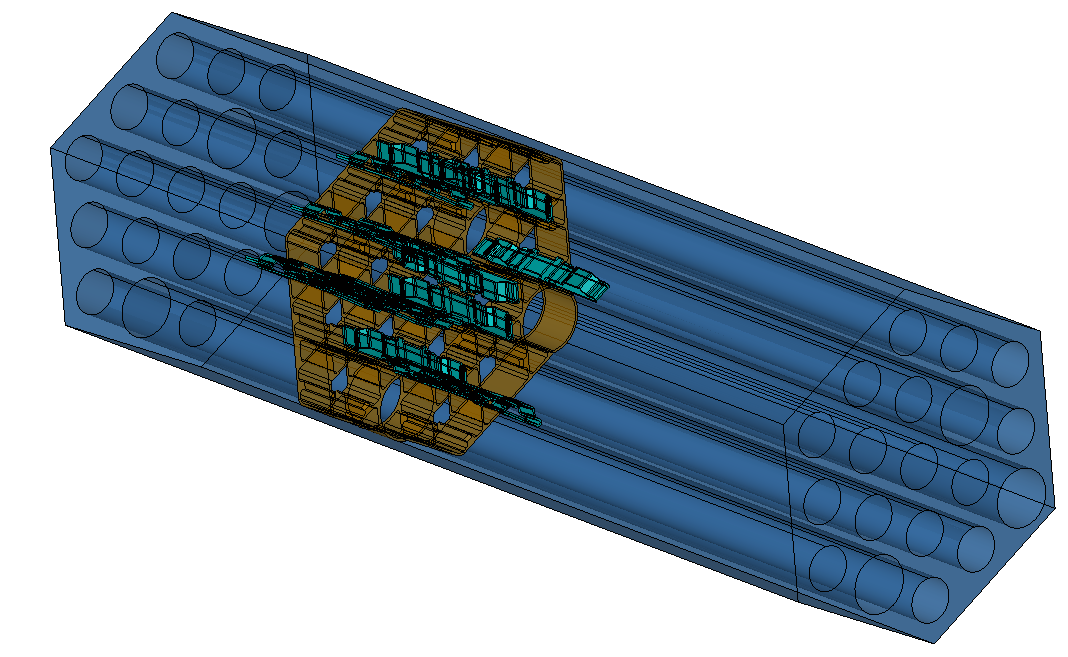
\includegraphics[width=5cm]{figsGEOM/salome_carem.png} \vspace{-3mm}
      \caption{Geometría construida en SALOME.}
    \end{figure}
  \end{minipage}
  \vspace{5mm}
  
  \begin{minipage}{0.425\textwidth}
     \begin{figure}
     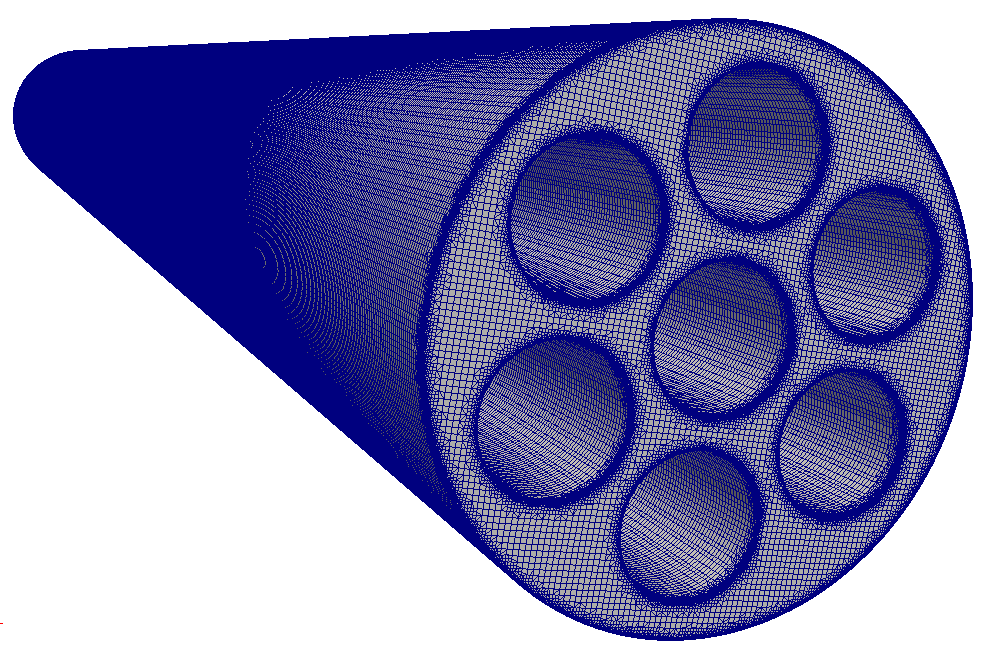
\includegraphics[width=4cm]{figsGEOM/OpenFOAM_atucha.png} \vspace{-3mm}
      \caption{Malla creada en OpenFOAM.}
    \end{figure}
  \end{minipage}
    \begin{minipage}{0.525\textwidth}
  \begin{block}{OpenFOAM}
    Conjunto de bibliotecas de C++, destinadas a crear aplicaciones que involucren la resolución de EDP.
    \begin{itemize}
    \item Generación de mallas hexahédricas.
    \item Resolución de ecuaciones RANS mediante FVM.
    \end{itemize}
  \end{block}
  \end{minipage}

    \note{\begin{itemize}
      \item SnappyHexMesh es una utilidad de OpenFOAM que permite generar mallas hexahédricas para geometrías arbitrarias. Su desempeño es muy bueno.
       \end{itemize}
    }

}


% =====================================================================================================
 \section{Geometría}
\frame{
  \frametitle{Geometría}
  \framesubtitle{Elemento combustible símil ATUCHA II}


  \begin{columns}
      \hspace{-1cm}
    \column{0.65\textwidth}
    \begin{minipage}[c][0.4\textheight][c]{\linewidth}
     \begin{figure}
       %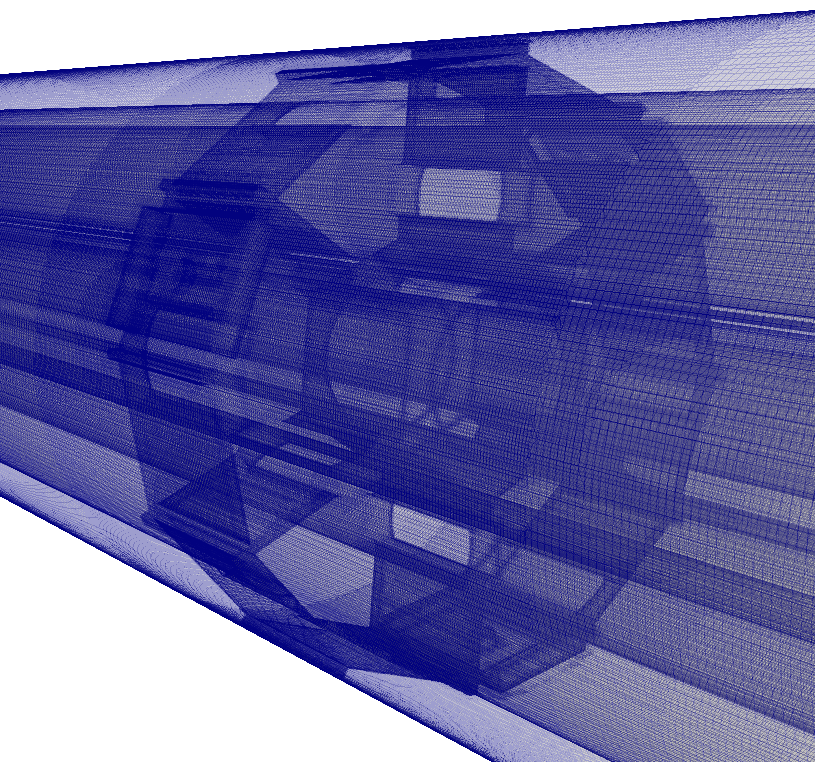
\includegraphics[width=0.55\linewidth]{figsATUCHA/atucha_mesh1a.png}
     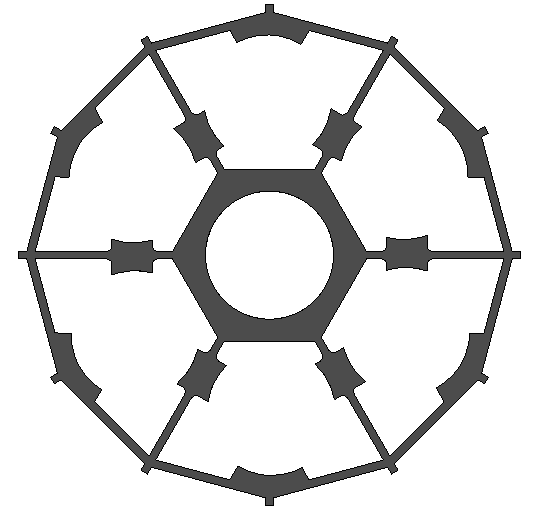
\includegraphics[width=0.525\linewidth]{figsATUCHA/2.png} \vspace{-3mm}
      \caption{Sección transversal del separador}
    \end{figure}
    \end{minipage}

    \vspace{0.5cm}
    \begin{minipage}[c][0.4\textheight][c]{\linewidth}
      \begin{figure}
        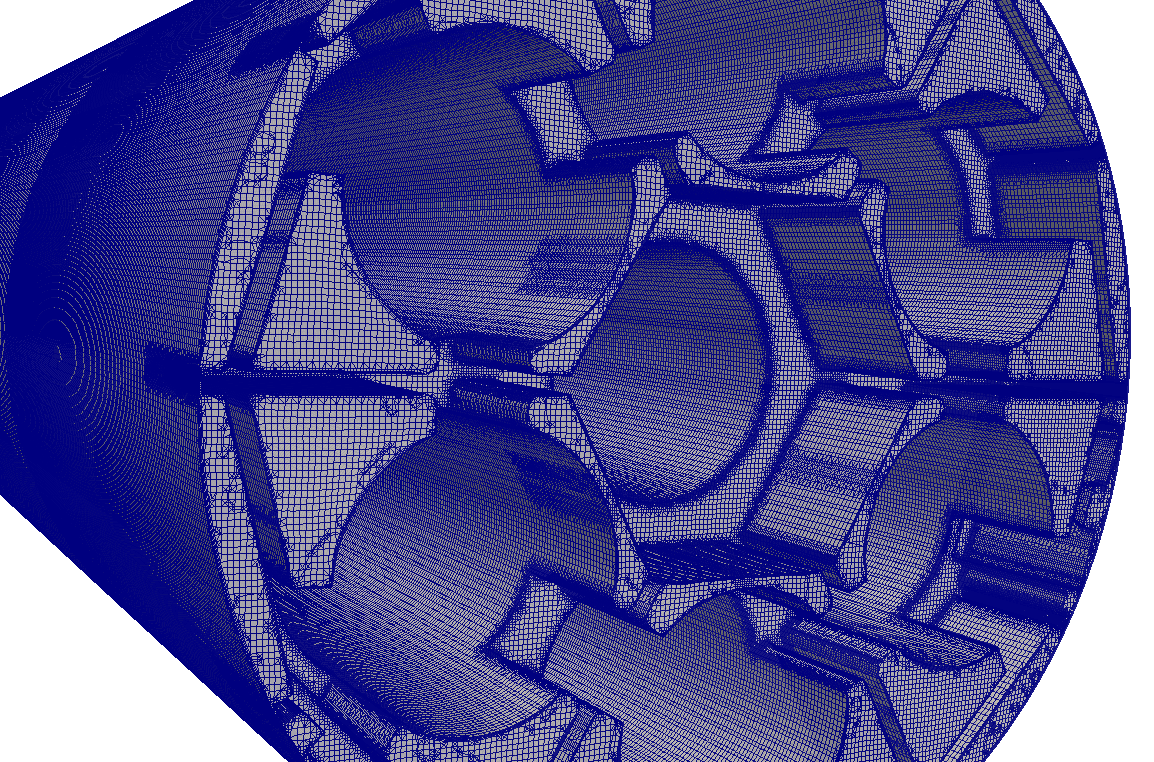
\includegraphics[width=0.65\linewidth]{figsATUCHA/atucha_mesh2a.png} \vspace{-3mm}
        \caption{Corte en el centro del separador.}
      \end{figure}
    \end{minipage}
    
    \column{0.5\textwidth}
    \begin{minipage}[c][0.4\textheight][c]{\linewidth}
      \begin{itemize}
      \item Símil CNAII 7 vainas.
      \item Malla de 14M de celdas.
      \item 4 capas adicionales en bordes.
      \end{itemize}
    \end{minipage}
    
    \begin{minipage}[c][0.5\textheight][c]{\linewidth}
      \begin{figure}
        \hspace{-1.5cm}   
        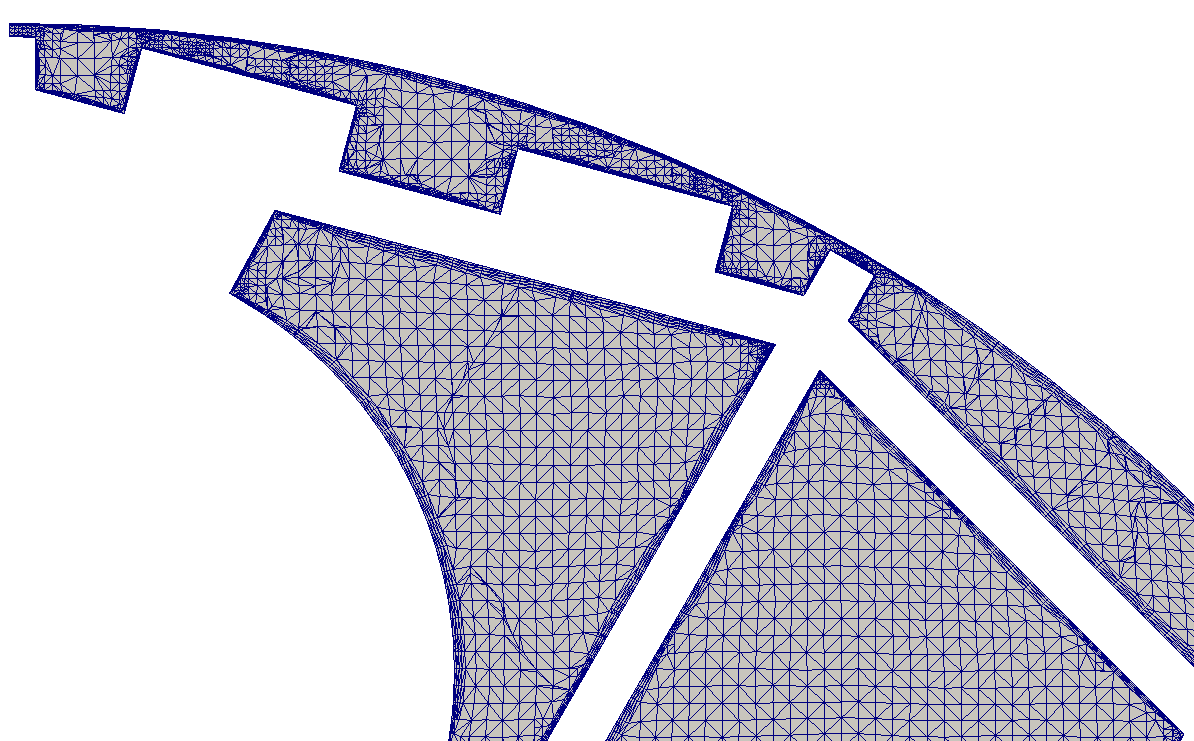
\includegraphics[width=0.95\linewidth]{figsATUCHA/atucha_mesh3a.png} \vspace{-3mm}
        \caption{Detalle de capas adicionales.}
        \end{figure}
    \end{minipage}
  \end{columns}

    \note{\begin{itemize}
      \item Esta geometría fue utilizada para realizar mediciones de pérdida de carga en el Laboratorio THI del CAB.
       \end{itemize}
    }
}



% ===========================================================================================================
\section{Resultados}
\subsection{Modelos de turbulencia}
\frame{
  \frametitle{Modelos de turbulencia}

    \begin{minipage}[c]{0.65\linewidth}
      \begin{itemize}
      \item Geometría: canal circular con 7 vainas.
      \item Condición de borde periódica en la dirección del flujo.
      \item Análisis de modelos de turbulencia:
      \end{itemize}
    \end{minipage}
    \begin{minipage}[c]{0.3\linewidth}
      \begin{figure}
        \center
      
\includegraphics[width=0.65\linewidth]{figsGEOM/geom_mod_turb.png} \vspace{-3mm}
      \caption{Sección transversal del canal analizado.}
    \end{figure}
    \end{minipage}
    
   \begin{table}[ht]
%      \setlength{\tabcolsep}{10pt}
        \centering
        \begin{tabular}{c c  c }
            \hline
            \bf Modelo & \bf CB   &  \bf Pendiente \\
            \hline
            \hline
            $k$ - $\omega$ SST    & k: kLowReWallFun, $\omega$: omegaWallFun  &  4354\\ % 4.364
            $k$ - $\omega$ SST    & k: fixedValue (0), $\omega$: omegaWallFun  &  4360\\ % 4.3702
            $k$ - $\omega$  & k: kLowReWallFun, $\omega$: omegaWallFun  &  4662 \\ % 4.6729
            $k$ - $\omega$  & k: fixedValue (0), $\omega$: omegaWallFun  &  4820 \\ %4.831
            Spallart Almaras & $\nu_t$: nutSpaldingWallFunction &  4840 \\ %4.851
            \hline
            Mediciones &  & 5509 \\
            \hline
        \end{tabular}
        \caption{Modelos de turbulencia estudiados.}
    \end{table}    

   \note{
     \scriptsize{
     \begin{itemize}
      \item kLowReWallFunction: provides a turbulent kinetic energy boundary condition for low and high Reynolds number flow cases.  (De Liu, ``A thorough description of how...'')
     \item omegaWallFun: provides constraint on turbulent specific disipation. Provides the combination of viscous and log equation. In OpenFOAM is a special wall function wich switch between viscous and logarithmic region according to the position of y+. In the intersection of the viscous sublayer and log-law region value is calculated through blending the viscous and log-law sublayer value.
     \item k-omega SST (hecho por Menter) is a model to be used in the sublayer of the boundary layer. The difference of this model from the other models is that it does not include damping functions and it is superior wilcox k-omega  model since it is more accurate. The k-epsiolon model is independent from the freestream values in the outer region of the boundary layer and Menter used the k-epsilon formulation to propose the new model.

       SST means shear stress transport. Menter noted two failings of the basic k-omega model. One minor, that it overpredicts the level of shear stress in adverse pressure-gradient boundary layers. One mayor, that it has spurious sensitivity to free-stream conditions.

       The model combines the k-omega turbulence model and K-epsilon turbulence model such that the k-omega is used in the inner region of the boundary layer and switches to the k-epsilon in the free shear flow.

      \item Nota sobre elección de Spallart Almaras
      \end{itemize}
}
   }
}

\subsection{EC ATUCHA}
\frame{
  \frametitle{Elemento combustible símil ATUCHA}
  \framesubtitle{Pérdida de carga}
  \begin{figure}[!htb]
    \center
    %\includegraphics[width=10cm]{figsATUCHA/US_DS.png}
    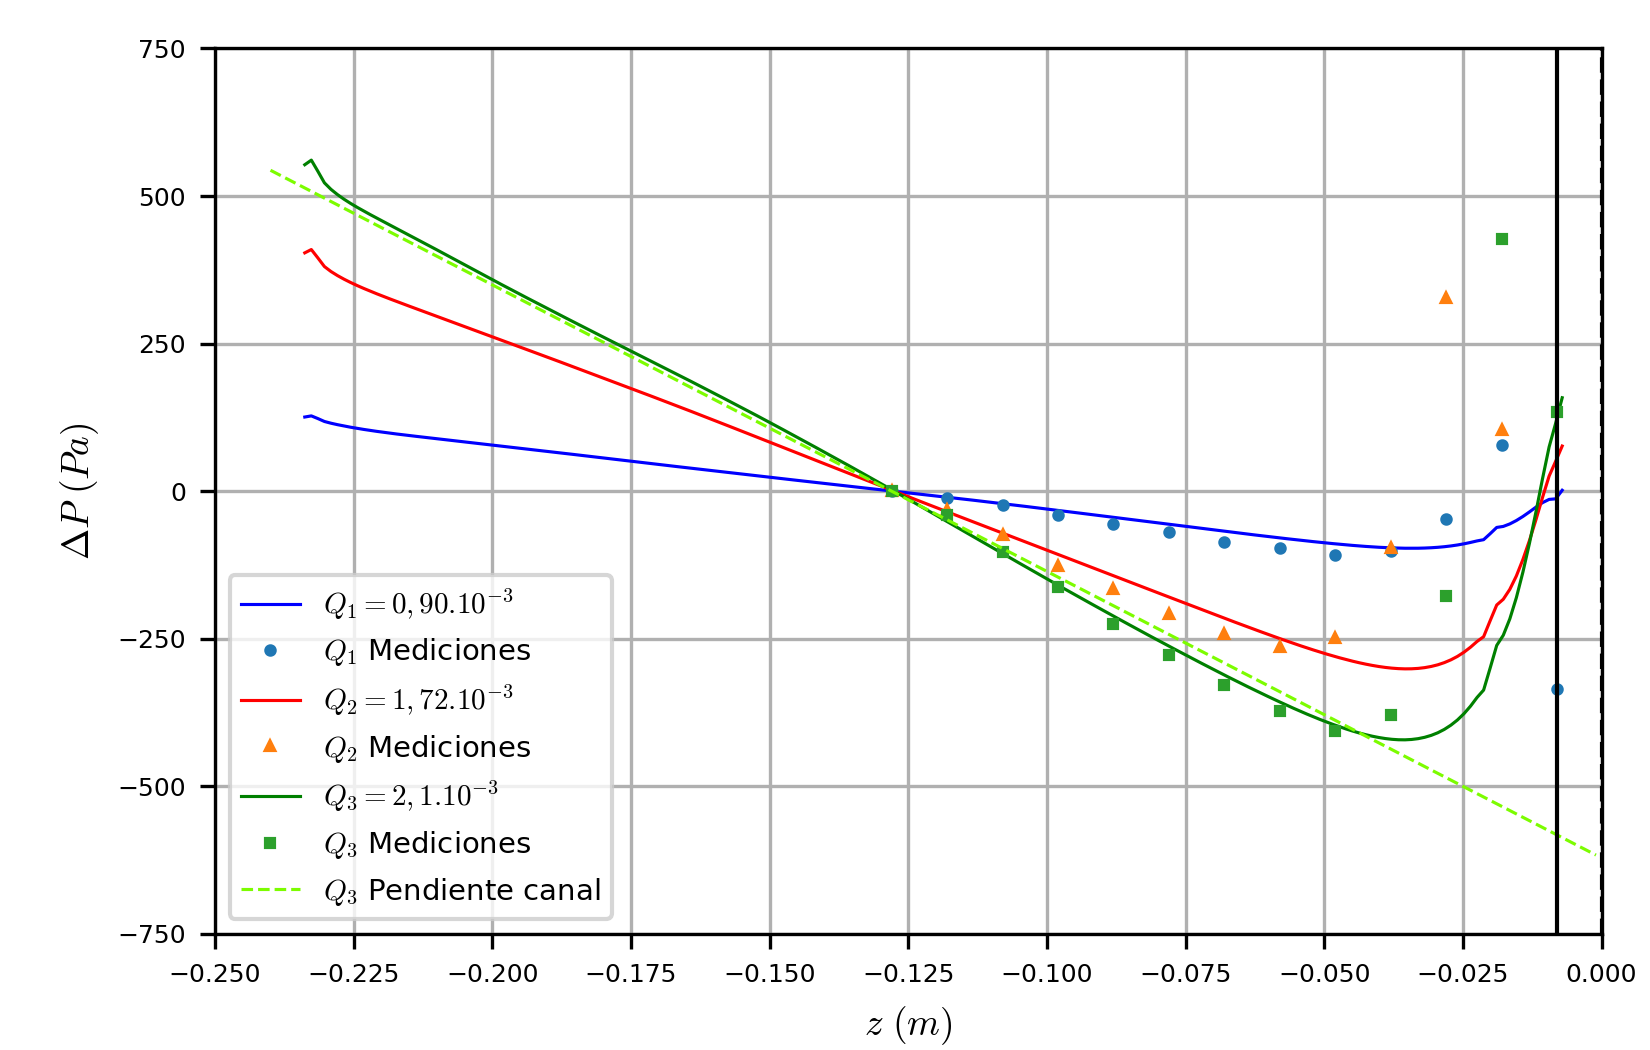
\includegraphics[width=10cm]{figsATUCHA/US.png}
  \end{figure}

}

\frame{
  \frametitle{Elemento combustible símil ATUCHA}
  \framesubtitle{Pérdida de carga}
  \begin{figure}[!htb]
    \center
    %% 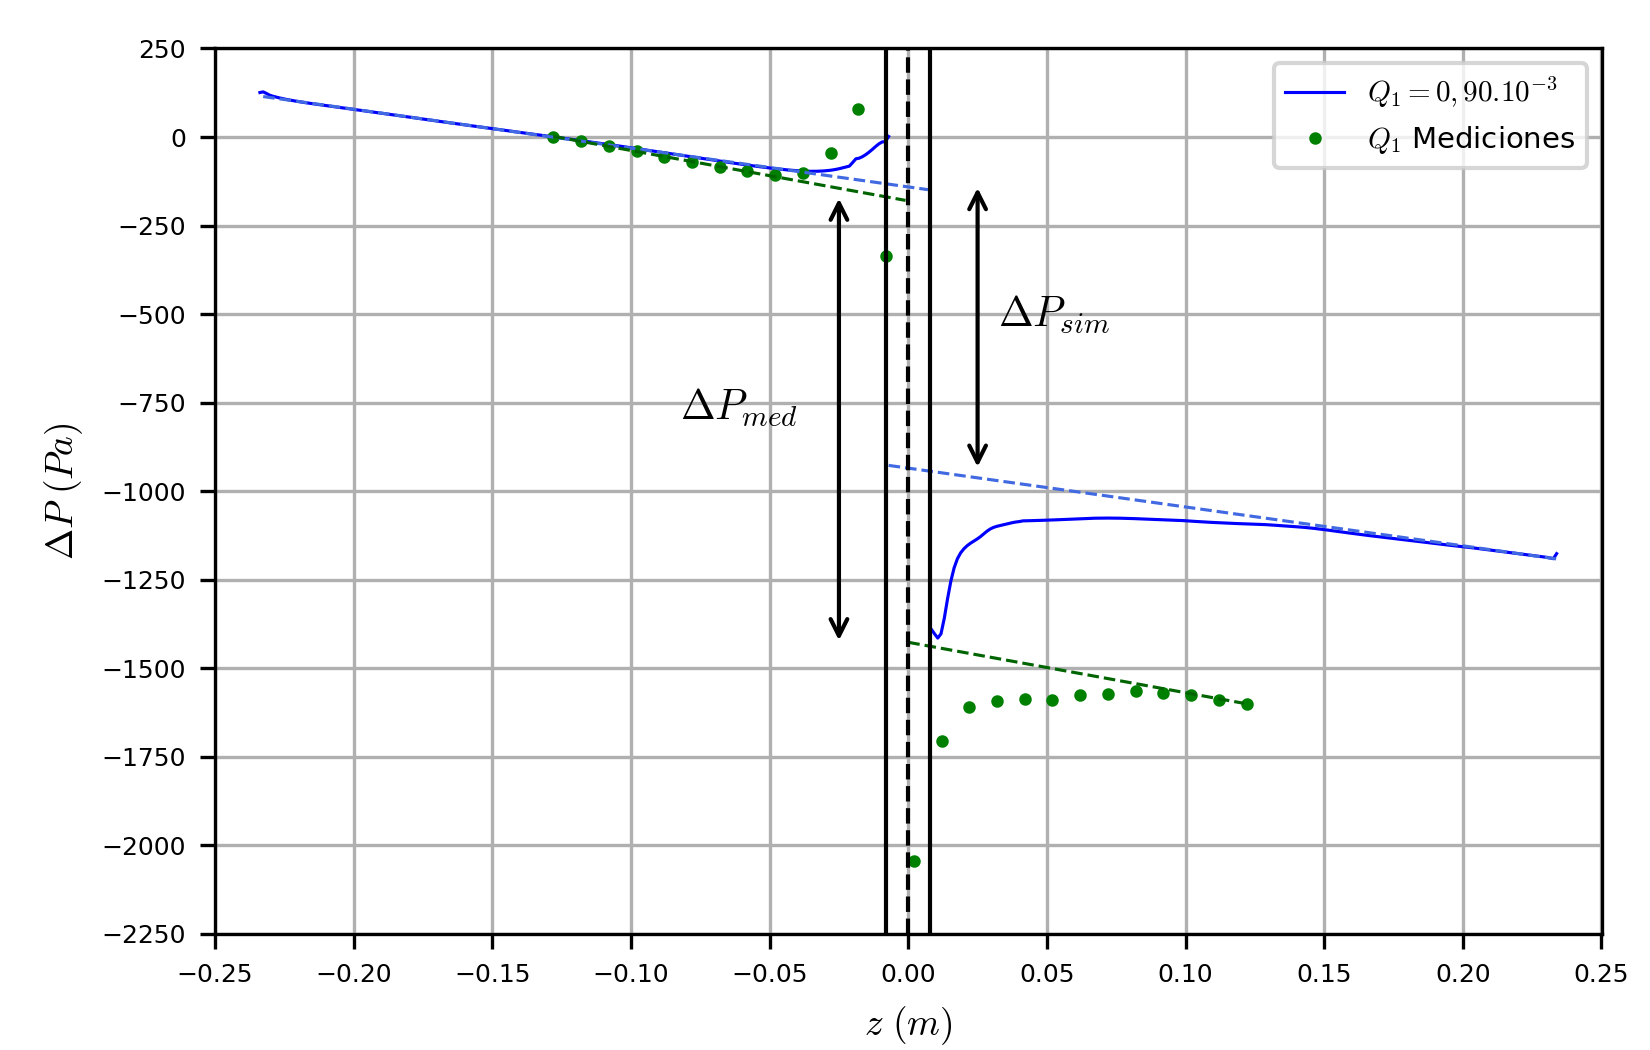
\includegraphics[width=8cm]{figsATUCHA/US_DS_fit_Q1.png}
    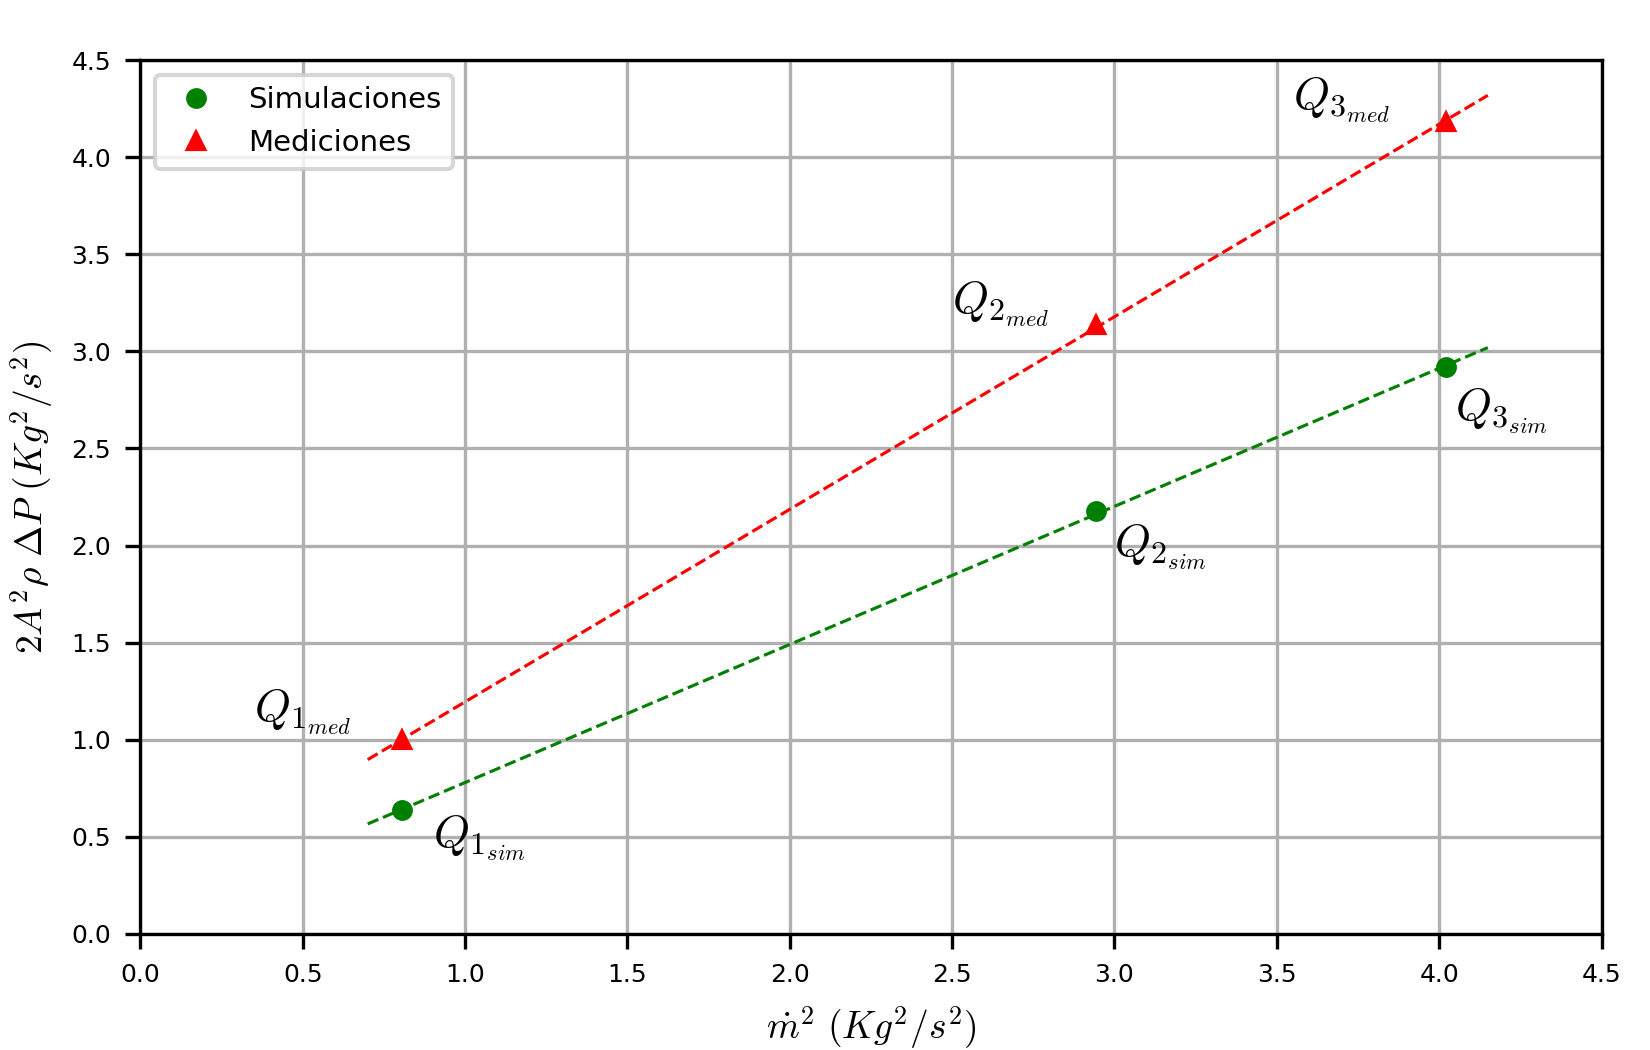
\includegraphics[width=8.5cm]{figsATUCHA/m_vs_DP.png}
  \end{figure}

  \begin{table}[ht]
        \centering
        \begin{tabular}{c | c | c | c }
            \bf Caudal $(m^3/s)$  & \bf $\Delta P_{sim}$  & \bf $\Delta P_{med}$ & \bf Diferencia (\%)  \\
            \hline
            \hline
            $Q_1=0.90 10^{-3}$ & 794.15  & 1246.43 & 36.3 \\
            $Q_2=1.72 10^{-3}$ & 2716.69 & 3910.64 & 30.5 \\
            $Q_3=2.01 10^{-3}$ & 3640.50 & 5220.35 & 30.3 \\
        \end{tabular}
        \caption{Valores de pérdida de carga local.}
        \label{tab:DP}
  \end{table}
  
}
\frame{
  \frametitle{Elemento combustible símil ATUCHA}
  \framesubtitle{Distribución de velocidad principal}

  \begin{textblock}{3}(-1,-3.5)
  \begin{figure}[!htb]
    \center
    \usetikzlibrary{arrows}
\begin{tikzpicture}[scale=0.01]

\draw [line width=0.5] (0,-235) -- (0,235) -- (50,235) -- (50,-235) -- cycle;
\fill[black!60!white] (0,-8) -- (0,8) -- (50,8) -- (50,-8) -- cycle;

\draw [line width=0.75, dashed] (-10,-200) -- (60,-200);
\node at (-30,-200) {\scriptsize{(f)}};

\draw [line width=0.75, dashed] (-10,-23) -- (60,-23);
\node at (-30,-35) {\scriptsize{(e)}};

\draw [line width=0.75, dashed] (-10,-15.5) -- (60,-15.5);
\node at (80,-15) {\scriptsize{(d)}};

\draw [line width=0.75, dashed] (-10,0) -- (60,0);
\node at (-30,0) {\scriptsize{(c)}};

\draw [line width=0.75, dashed] (-10,15.5) -- (60,15.5);
\node at (80, 25.50) {\scriptsize{(b)}};

\draw [line width=0.75, dashed] (-10,200) -- (60,200);
\node at (-30,200) {\scriptsize{(a)}};

\draw [->,>=stealth',line width=1.25] (25,-250) -- (25,-300); 

%\draw [line width=0.5] (-235,0) -- (235,0) -- (235,50) -- (-235,50) -- cycle;
%\fill[black!60!white] (-8,0) -- (8,0) -- (8,50) -- (-8,50) -- cycle;
%\draw [line width=0.75, dashed] (-200,-10) -- (-200,60);
%\node at (-200,-30) {\scriptsize{(a)}};
%\draw [line width=0.75, dashed] (-15.5,-10) -- (-15.5,60);
%\node at (-25.5,-30) {\scriptsize{(b)}};
%\draw [line width=0.75, dashed] (0,-10) -- (0,60);
%\node at (0,-30) {\scriptsize{(c)}};
%\draw [line width=0.75, dashed] (15.5,-10) -- (15.5,60);
%\node at (25.5,-30) {\scriptsize{(d)}};
%\draw [line width=0.75, dashed] (200,-10) -- (200,60);
%\node at (200,-30) {\scriptsize{(e)}};

\end{tikzpicture}
  \end{figure}
  \end{textblock}
  
  \begin{textblock}{12}(1.25,-6.5)
  \begin{figure}[ht]
        \centering
        %\begin{subfigure}[t]{0.45\textwidth}
            \centering
            \subfloat[]{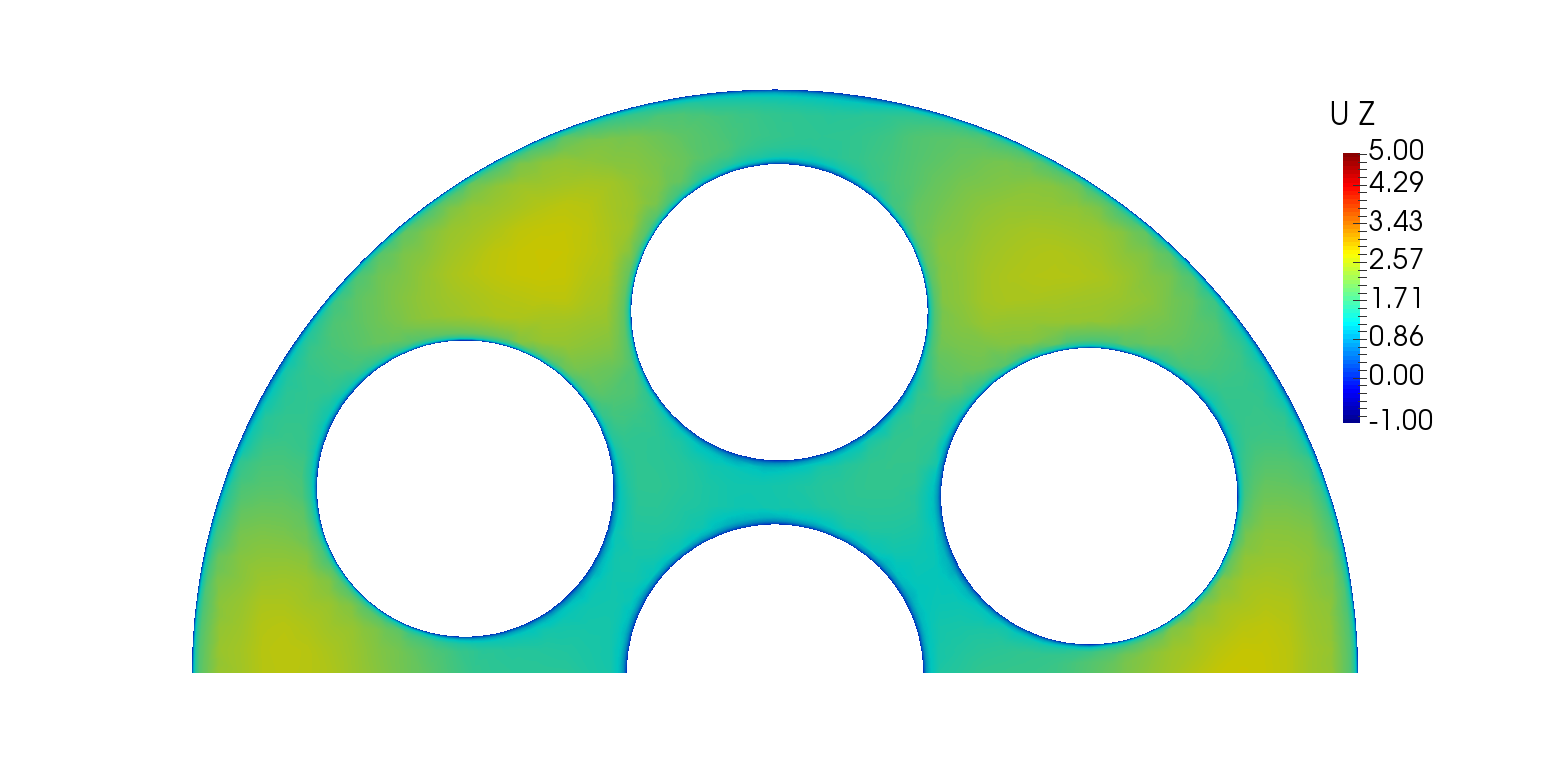
\includegraphics[width=0.5\textwidth]{figsATUCHA/vel/U_020US.png}}
            \subfloat[]{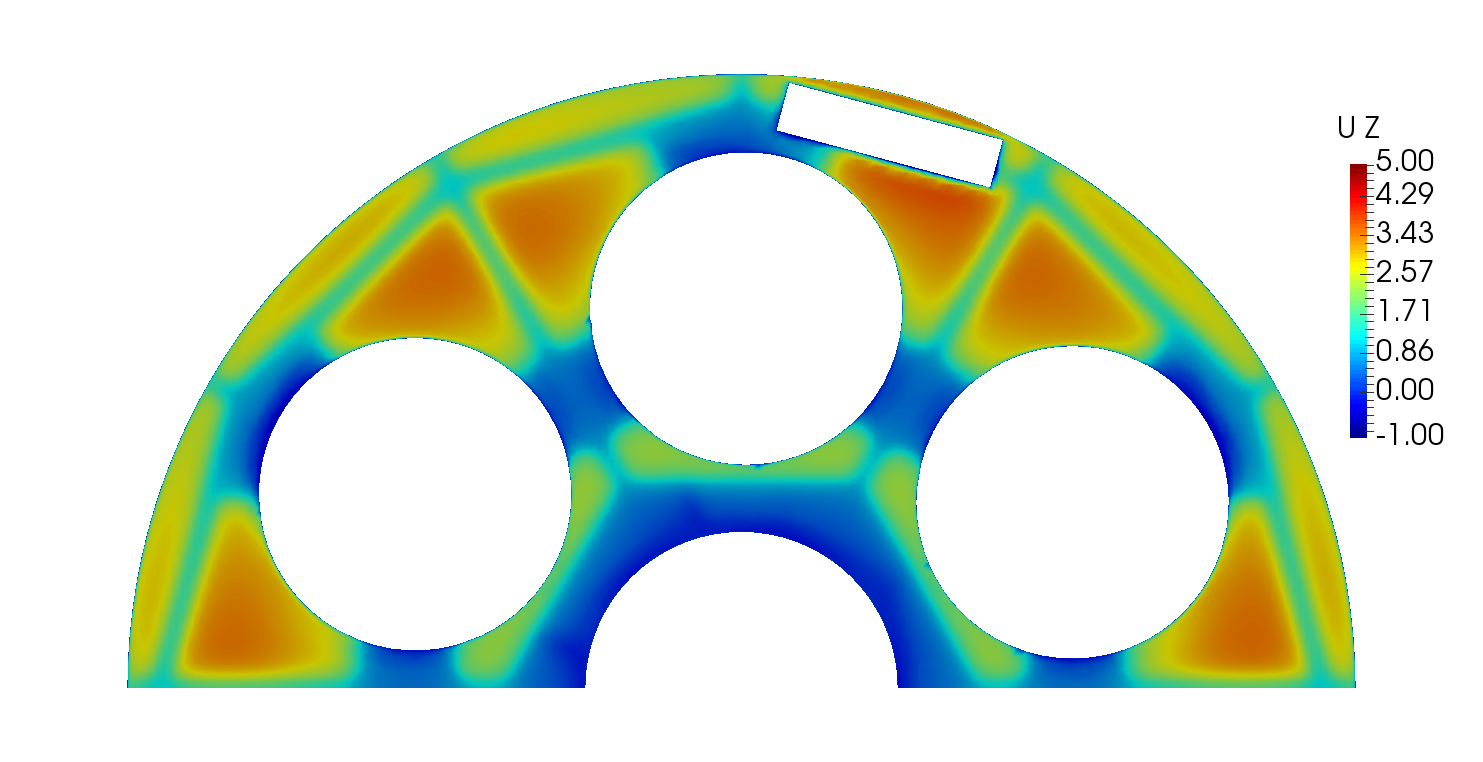
\includegraphics[width=0.45\textwidth]{figsATUCHA/vel/U_00075US.png}}
            \vspace{-5mm}
            
            \subfloat[]{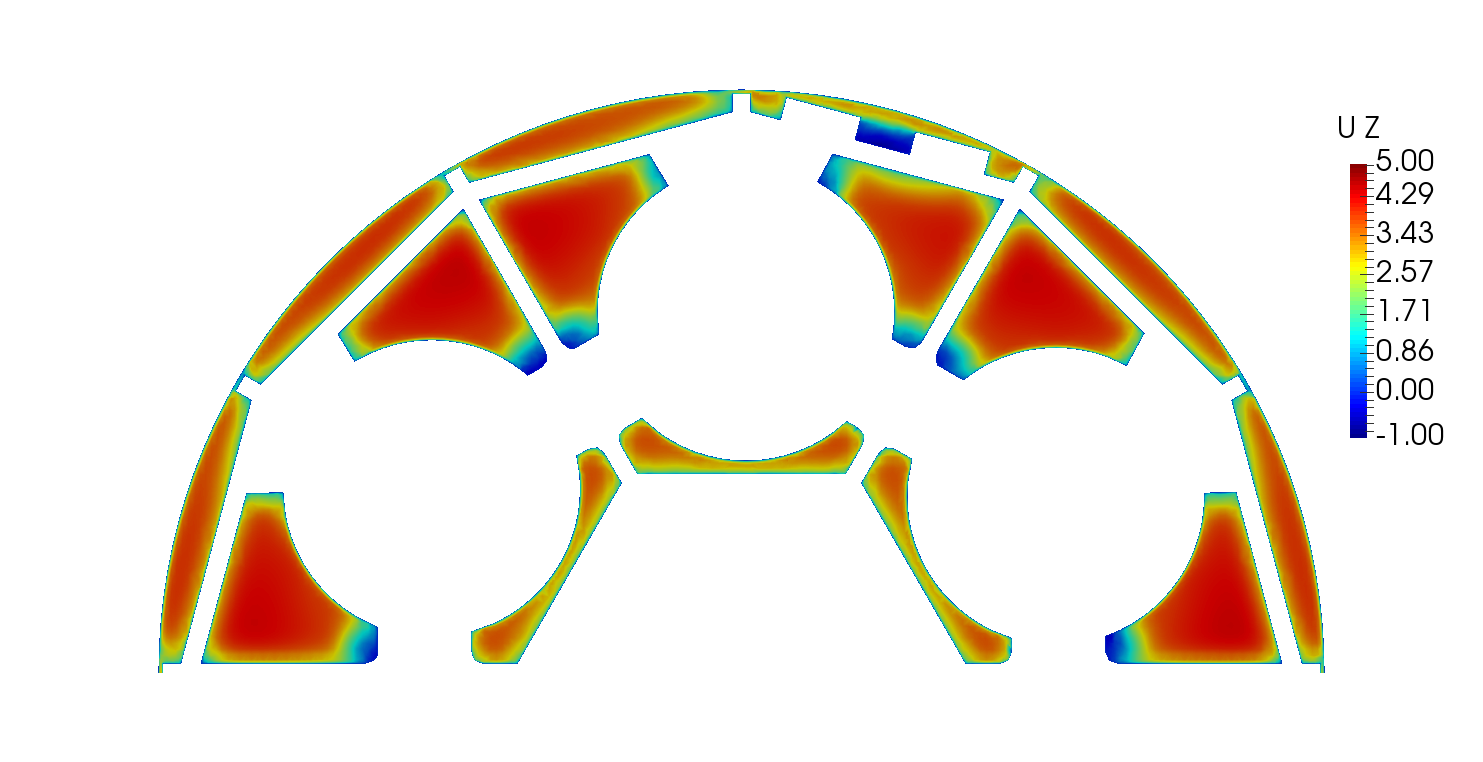
\includegraphics[width=0.45\textwidth]{figsATUCHA/vel/U_half.png}}
            \subfloat[]{ 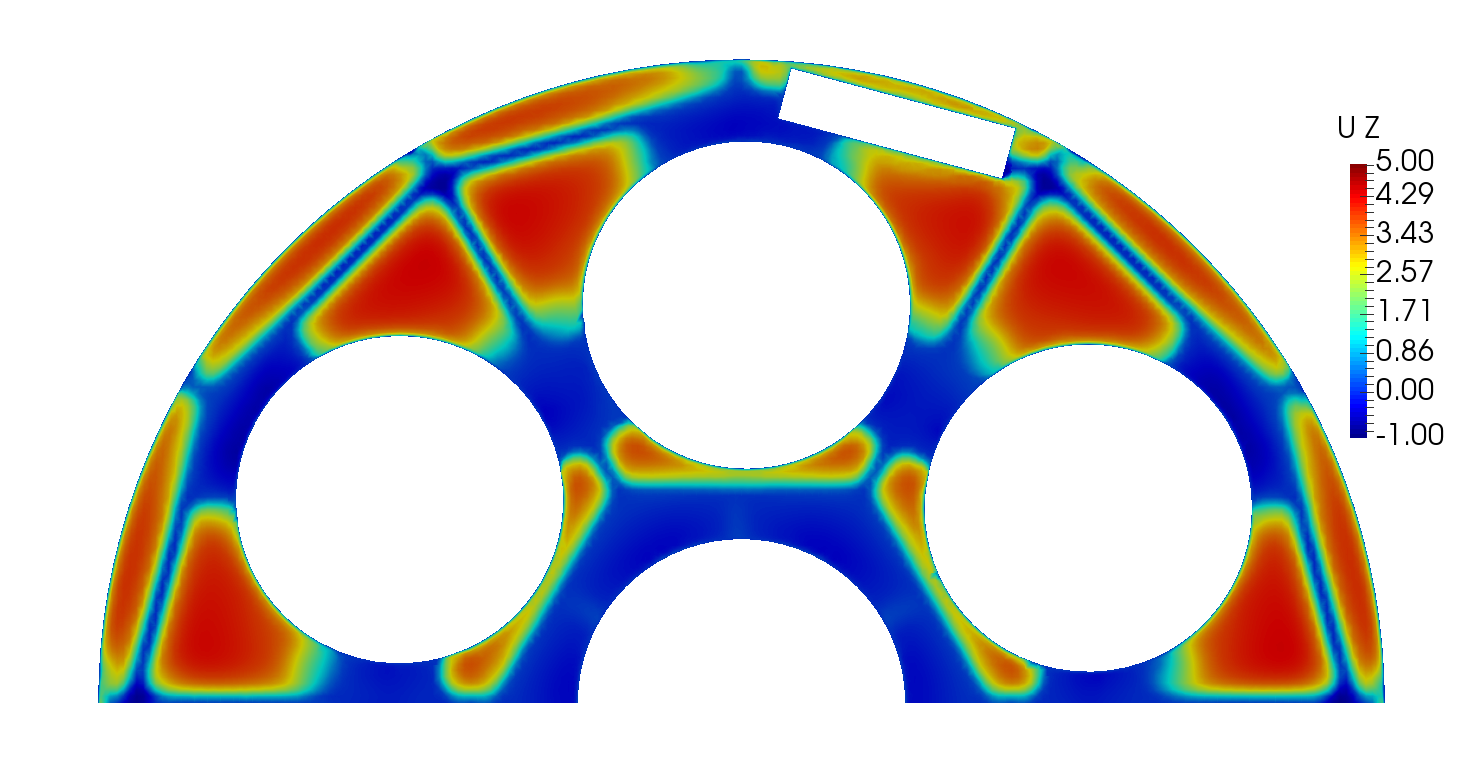
\includegraphics[width=0.45\textwidth]{figsATUCHA/vel/U_00075DS.png}}
            \vspace{-5mm}
             
            \subfloat[]{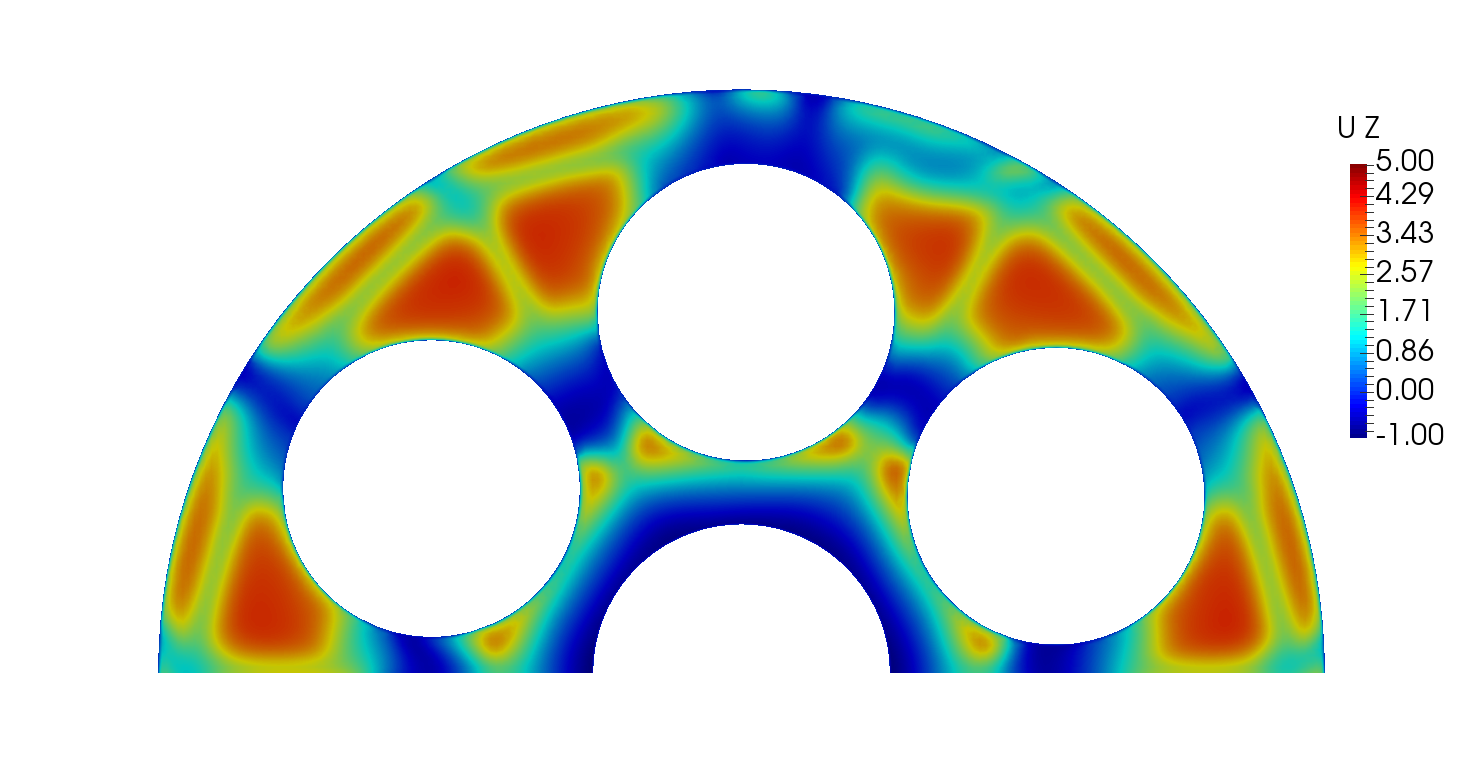
\includegraphics[width=0.45\textwidth]{figsATUCHA/vel/U_0015DS.png}}
            \subfloat[]{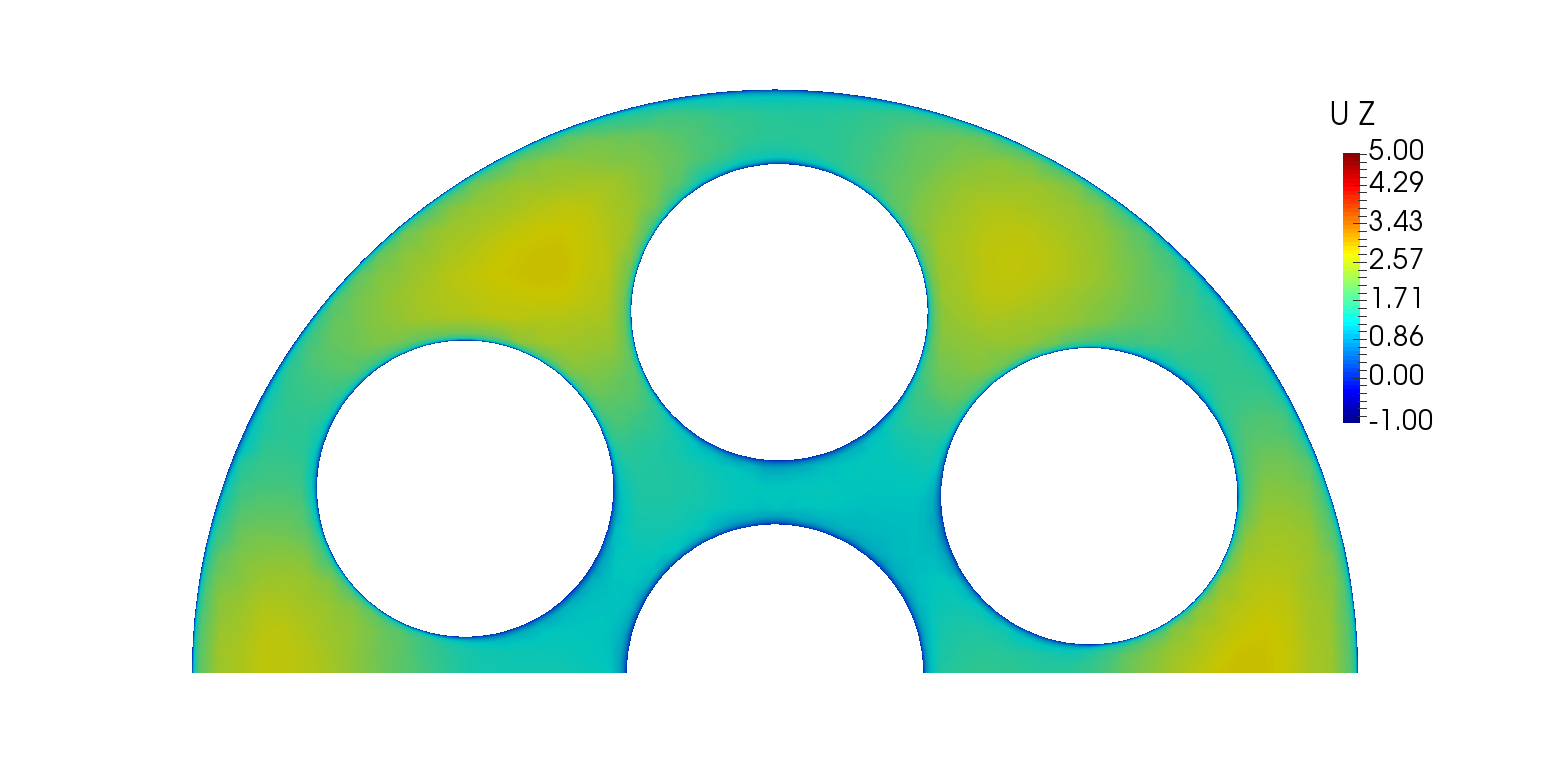
\includegraphics[width=0.5\textwidth]{figsATUCHA/vel/U_020DS.png} \vspace{-3mm}}
        \caption{Distribución de la velocidad principal en secciones transversales: a) a 200mm US del separador, b) a 7.5mm US del separador, c) en la mitad del separador, d) a 7.5mm DS del separador, e) a 15mm DS del separador y f) a 200mm DS del separador.}
  \end{figure}
  \end{textblock}
}

% =====================================================================================================
\frame{
  \frametitle{Geometría}
  \framesubtitle{Elemento combustible símil CAREM}
  
%  \vspace{-0.25cm}
  \begin{columns}
    \column{0.65\textwidth}
    \begin{minipage}[c][0.4\textheight][c]{\linewidth}
     \begin{figure}
        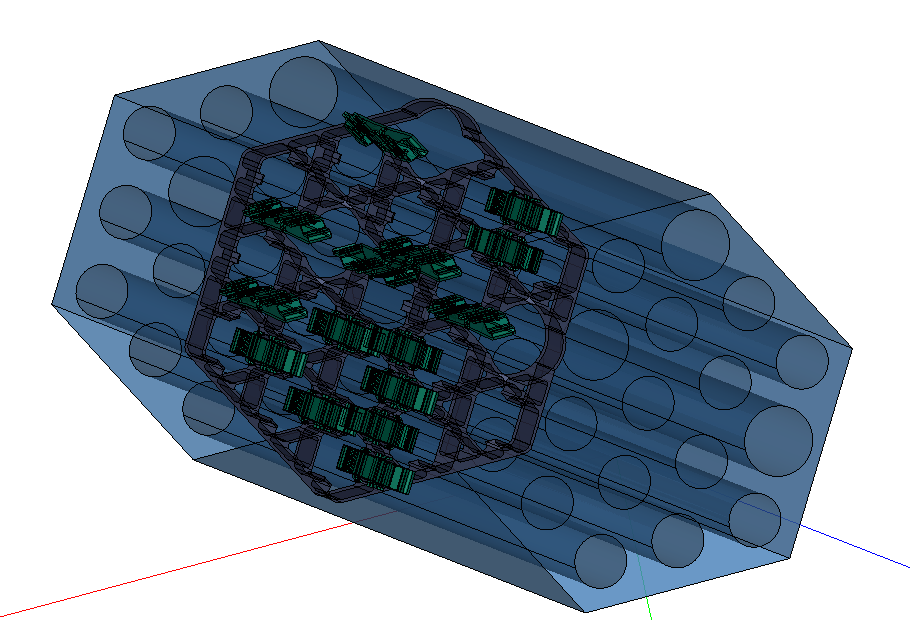
\includegraphics[width=0.85\linewidth]{figsCAREM/CAREM3.png} \vspace{-3mm}
        \caption{Geometría completa.}
    \end{figure}
    \end{minipage}

    %\vspace{0.5cm}
    \begin{minipage}[c][0.4\textheight][c]{\linewidth}

      \begin{itemize}
      \item Símil CAREM de 16 vainas y 3 tubos de control.
      \item Malla de 53M de celdas.
      \item 4 capas adicionales en bordes.
      \end{itemize}
      
    \end{minipage}
    
    \column{0.45\textwidth}
    \begin{minipage}[c][0.4\textheight][c]{\linewidth}
      \begin{figure}
     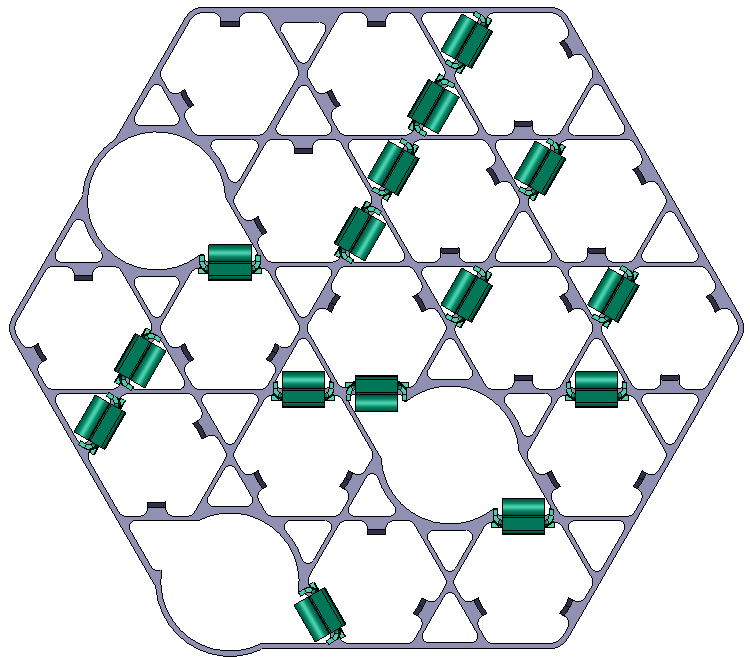
\includegraphics[width=0.8\linewidth]{figsCAREM/CAREM1.png} \vspace{-3mm}
      \caption{Vista de separador y resortes.}
      \end{figure}
    \end{minipage}
    
    \begin{minipage}[c][0.5\textheight][c]{\linewidth}
      \begin{figure}
        %\hspace{-1.5cm}   
        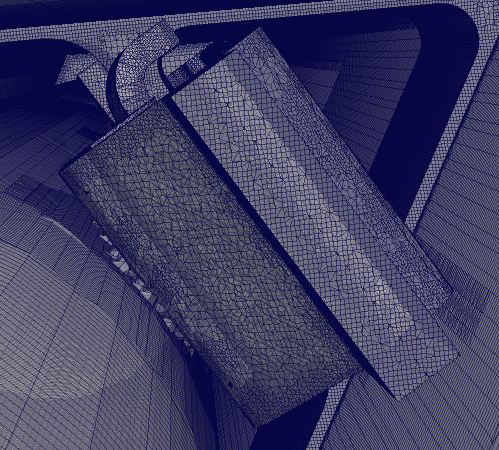
\includegraphics[width=0.75\linewidth]{figsCAREM/mesh_detalle3.png} \vspace{-3mm}
        \caption{Detalle de malla en resorte.}
        \end{figure}
    \end{minipage}
  \end{columns}
 
}

% ==========================================================================================================
\subsection{EC CAREM}
\frame{
  \frametitle{Elemento combustible símil CAREM}
  \framesubtitle{Pérdida de carga}
   \begin{figure}
      \includegraphics[width=10cm]{figsCAREM/US_DS.png} %\vspace{-3mm}
     % \caption{Sección transversal del separador}
   \end{figure}

   \note{Gráfico a revisar por Ezequiel}
}

\frame{
 \frametitle{Elemento combustible símil CAREM}
  \framesubtitle{Distribución de velocidades}
   \begin{figure}
       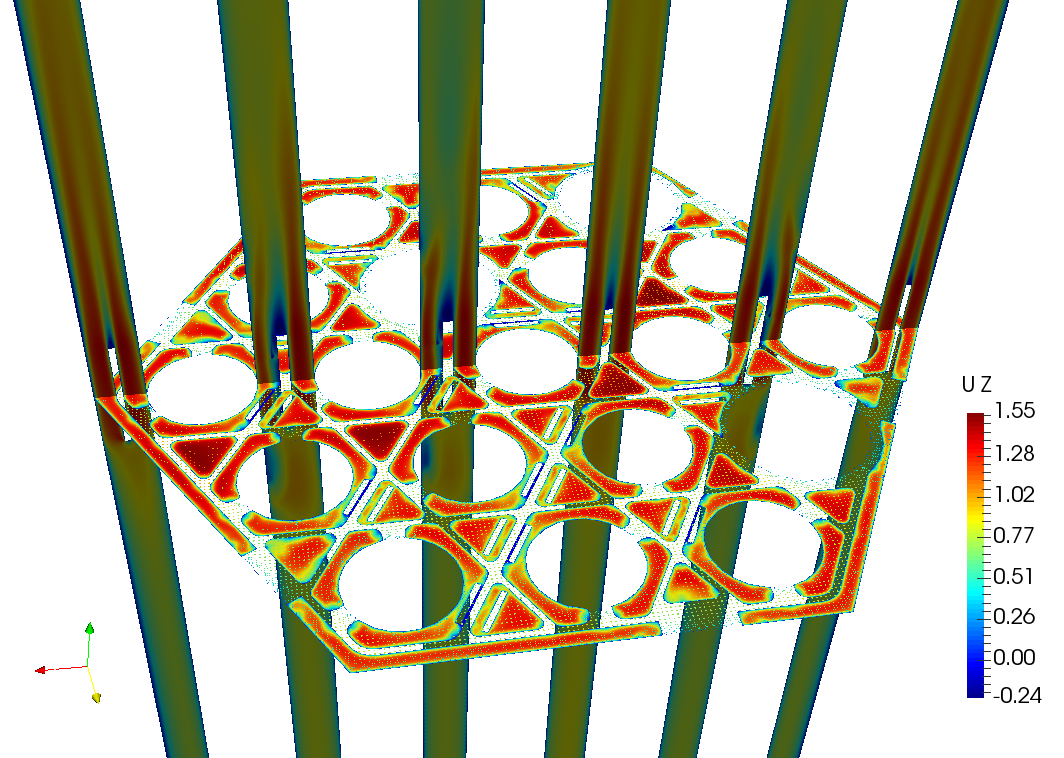
\includegraphics[width=10cm]{figsCAREM/CAREM4.png} %\vspace{-3mm}
       \caption{Vista de cortes: velocidad principal en el plano transversal en el centro del separador y en un plano longitudinal. Flujo de abajo hacia arriba.}
   \end{figure}
  
}

\frame{
 \frametitle{Elemento combustible símil CAREM}
  \framesubtitle{Distribución de velocidades}
   \begin{figure}
       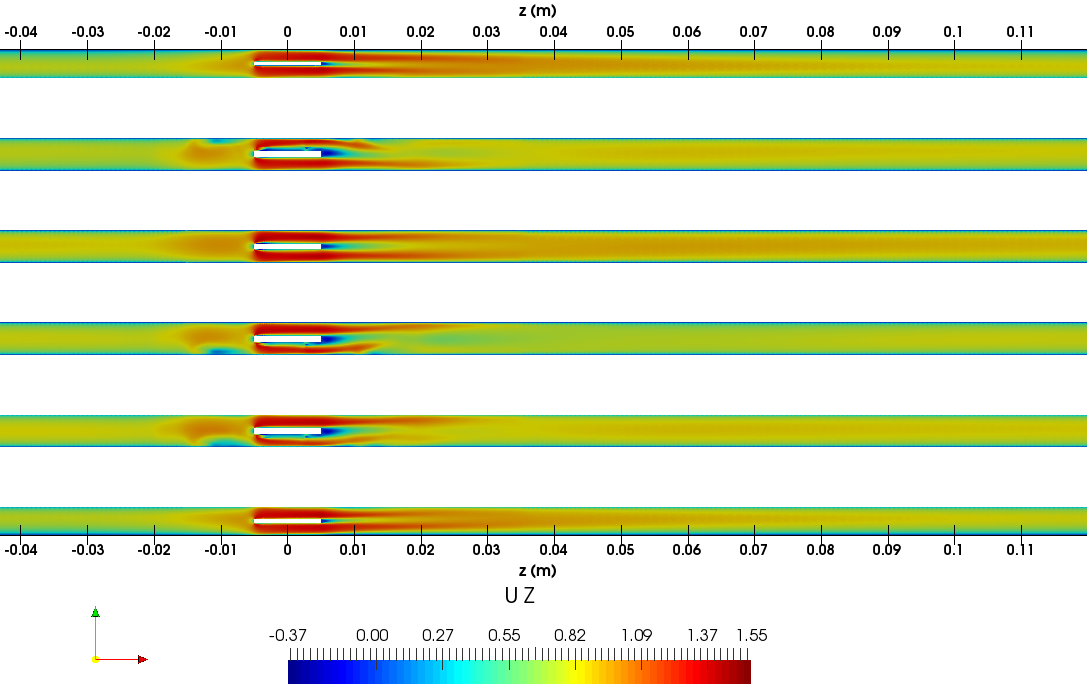
\includegraphics[width=10cm]{figsCAREM/CAREM6.png} %\vspace{-3mm}
       \caption{Velocidad principal en un plano longitudinal. Flujo de izquierda a derecha.}
   \end{figure}
  
}


\section{Conclusiones}
\frame{
  \frametitle{Conclusiones}

  \begin{itemize}
    \item Se llevaron a cabo simulaciones RANS en OpenFOAM.
    \item Las geometrías se mallaron con la herramienta SnappyHexMesh de OpenFOAM.
    \item Se realizó un análisis previo de varios modelos de turbulencia en un canal simple.
    \item Se calculó la pérdida de carga en un EC símil CNAII de 7 vainas y se comparó con mediciones experimentales.
      \begin{itemize}
      \item Similares pérdidas de carga longitudinales.
      \item Diferencias del 30\% en las pérdidas de carga locales.
      \end{itemize}
    \item Se realizó el cálculo de un EC símil CAREM de 16 vainas.
  \end{itemize}

  \note{Estas conclusiones me parecen un poco incompletas.}
}

\frame[plain]{
  \begin{textblock}{15}(3.75,1.25)
    \normalsize{¡Gracias por su atención!}
  \end{textblock}
  \begin{textblock}{15}(1.5,5)
    \normalsize{ XXIII Congreso sobre Métodos Numéricos y sus Aplicaciones}
  \end{textblock}
  \begin{textblock}{5}(-0.75,4.25)
    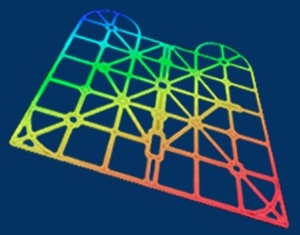
\includegraphics[width=1.5cm]{figuras/ENIEF2017.png}
  \end{textblock}
  
  %% \begin{textblock}{5}(5,0)
  %%   
\includegraphics[width=1.25cm]{figuras/CNEA.jpg}
  %% \end{textblock}
}


\end{document}

